\documentclass[../Notebook.tex]{subfiles}
\begin{document}

\chapter{11/27/2025 Exploration of the Metal Oxide Substrate (MOS) Sensor}

Discussion regarding the metal oxide substrate (MOS) sensors is had with its possible uses and calibrations as well as preliminary code and data collected from that code are shown. 

\hfill \break
\noindent Keywords: metal oxide substrate (MOS) sensor\index{metal oxide substrate (MOS) sensor}, MQ-135\index{MQ-135}, MQ-9\index{MQ-9}, LM393 comparator\index{LM393 comparator}, volatile organic compounds (VOCs)\index{volatile organic compounds (VOCs)}

\section{Introduction}

To determine the chemical makeup of the air that we breathe every day, I want to measure the amount of volatile organic compounds (VOCs) found in the steam being released from pipes all around the College of Science and Mathematics building. To this end, I want to employ something known as a metal oxide semiconductor (MOS) sensor that can measure the amount of various chemicals in the air. The MOS sensor operates on a straightforward principle: A substrate is heated to form an outer oxide layer - in this case, the substrate is tin (Sn) which forms SnO$_2$ when heated - and when reducing gasses - i.e. carbon monoxide (CO), carbon dioxide (CO$_2$), alcohol (C$_2$H$_5$OH), nitrous oxide (NO$_2$), ammonia (NH$_3$) - come nearby the substrate, the oxygen in the substrate-oxide is removed. This removal of oxygen molecules causes free electrons to move through the substrate and change the resistance of the sensor. This change in resistance is proportional to the amount of reducing gas present in the sample\footnote{For a brief overview of MOS sensors and the related chemistry \href{https://sensorsandtransmitters.com/a-brief-introduction-to-mos-sensors-and-their-applications/}{check here}.\label{mosfoot}}. These sensors are quite sensitive to temperature and humidity\footnote{This makes sampling steam particularly challenging…} and have other limiting factors such as the lack of selectivity in the gas sampled and baseline drift over time. That being said, the low cost, sensitivity, low power consumption, and relatively long lifespan of 5-10 years (for reference see footnote \ref{mosfoot}) make it an appealing option for gas sampling especially when compared to mobile mass spectroscopy systems that can cost upwards of \$80,000.

\section{Materials and Methods}

\subsection{The MOS Sensor}
\href{https://www.winsen-sensor.com/d/files/PDF/Semiconductor%20Gas%20Sensor/MQ135%20(Ver1.4)%20-%20Manual.pdf}{The MOS sensor itself} is a small roughly 2cm diameter $\times$ 2cm tall IC that contains a heating element, the Sn substrate, a grating that prevents debris accumulation, and six pins. \href{https://www.digikey.com/en/products/detail/olimex-ltd/SNS-MQ135/21662411?gclsrc=aw.ds&gad_source=1&gad_campaignid=20232005509&gbraid=0AAAAADrbLlhcj_2Qw_LwmJ1b6gtDedV1U&gclid=Cj0KCQiAiqDJBhCXARIsABk2kSkWHiFMI8xYM0RcLsyE9FJbAhpZYWMrR9DvBRDUFAZiyZroWf-9P6waApl1EALw_wcB}{The MOS sensors I’m working with} come on a daughter board that, while containing several resistors and capacitors that presumably are required for operation along with a power LED indicator as seen in Figure \ref{MOSoverview}, which can output signal using a couple of different operations depending on what pin you elect to read from (see Figure \ref{MOSpinout}). The first operation is that it can serve as an alarm through its digital output. This mode uses a \href{https://www.ti.com/lit/ds/symlink/lm393b.pdf?ts=1764190524626}{LM393 comparator} to detect when a reference voltage exceeds a certain level. As described \href{https://en.wikipedia.org/wiki/Comparator}{here} the comparator returns LOW when the input voltage is below a certain threshold and returns HIGH when the input voltage exceeds that amount. In the case of these sensors, the reference voltage is set by a potentiometer. 

\begin{figure}[h!]
	\centering
	\begin{subfigure}{.45\textwidth}
		\centering
		\includegraphics[width=.9\linewidth]{../figures/mq135-air-quality-sensor-overview }
		\caption{Overview of the MQ135 MOS sensor.}
		\label{MOSoverview}
	\end{subfigure}%
	\begin{subfigure}{.45\textwidth}
		\centering
		\includegraphics[width=.9\linewidth]{../figures/mq135-air-quality-sensor_pinout }
		\caption{Pinout diagram of the MQ 135 MOS sensor.}
		\label{MOSpinout}
	\end{subfigure}
	\label{MOSpics}
	\caption{Pictures of the MQ 135 MOS sensor attached to its daughter board.}
\end{figure}

The second method of operation is the analog output. The analog output returns the raw analog signal coming from the MOS sensor itself. The meaning of this signal is significantly more challenging to resolve. 

Regardless of the method of data acquisition, the MOS sensor must be treated with special care. Specifically the heating of the MOS sensor must be allowed to take place before measurements are allowed to take place. This typically takes a minute or two, but the datasheets say that for long-term storage of 6+ months the sensor must be ``aged’’ for ``no less than 168 hours’’ before accurate measurements can be made.

\subsection{MOS Sensor End-User Calibration}
The \href{https://www.olimex.com/Products/Components/Sensors/Gas/SNS-MQ135/resources/SNS-MQ135.pdf}{datasheet} for the MQ135 shows a calibration curve as seen in Figure \ref{moscalone} below which appears to show how the resistance of the sensor ($R_s$) changes as a function of different \textit{known} gas concentrations. If we link these calibration curves with the fact that nowhere in the datasheet does it provide a simple conversion factor, the sensor must be end-user calibrated for precise operation. One could simply read the graph shown if Figure \ref{moscalone} and derive the ratio of resistance to ppm measurements, but that would, at best, be a ``hand grenade’’ kind of measurement as opposed to a ``scalpel’’. 

\begin{figure}[h!]
    \centering
    \includegraphics[width=.8\linewidth]{../figures/MOS_calibrationOne}
    \caption{A calibration curve of the MOS sensor is shown along with its original caption to the right of the figure.}
    \label{moscalone}
\end{figure} 

To my knowledge, there doesn’t exist a single method for calibration of the MOS sensor. Before designing a template for calibration, we must keep a couple of factors in mind. The first factor in calibration design is the temperature and humidity. There must be a consideration of temperature and humidity regulation in the test chamber. I think a temperature and humidity sensor such as \href{https://www.digikey.com/en/products/detail/dfrobot/DFR0067/6588511}{the DHT11} (\href{https://www.mouser.com/datasheet/2/758/DHT11-Technical-Data-Sheet-Translated-Version-1143054.pdf?srsltid=AfmBOooFRUztTnORkx4zQJWn4xbR5OOOAmrtbQ5FeJjtOQg0ZrL9Erp_}{datasheet available here}) could be employed to track the temperature and humidity during such calibrations. We must also devise a strategy for calculating the resistance of the sensor at the given temperature and humidity. According to this \href{https://projecthub.arduino.cc/ArduinoKoen/co2-monitor-57bbce}{(seemingly) well thought out post on the Arduino project hub}, we can calculate the resistance of the sensor by the following equation.
\begin{equation}
	Rdg = \frac{1024\cdot R_{\text{ref}}}{ R_{\text{ref}}+ R_{\text{s}}} \quad \xrightarrow \quad R_{\text{s}} = \left(\frac{1024}{Rdg} - 1\right) R_{\text{ref}}
\end{equation}

In the previous equation, $Rdg$ is the reading coming from the sensor, $R_{\text{ref}}$ is a reference resistance (assume STP, a given PPM, and ``clean air'' for this baseline reference resistance), and the 1024 - I believe - has to do with the Arduino's 10-bit ADC. It is noteworthy that there is no conversion from ``ADC step'' to voltage. Calibration strategy can be outlined by the following:

\begin{enumerate}
	\item Build a MOS, temperature, \& humidity sensor all-in-one such that the arduino can easily talk to all of the components at once.
	\item While controlling for the temperature and humidity, introduce known gas concentrations into an airtight chamber measuring the PPM of the gas by known, calibrated tools.
	\item Measure the sensor resistance as a function of the PPM, temperature, and humidity.
	\item Repeat measurements for a range of gas concentrations.
	\item Repeat measurements for a range of temperature and humidity conditions.
\end{enumerate}

Maybe there are other ways to accomplish this that don't involve thousands of dollars of high-speed lab equipment, but that's the best idea I have for now. Regardless of precision calibration the sensors will still produce a voltage and can be used to track relative increases in gas concentrations.

\subsection{The Circuit}

The current circuit I am using is seen in Figure \ref{moscircone}. I am borrowing the circuit from another professor, so it has multiple MOS sensors of different series on it. The actual connections required for the MOS sensor to function are seen in Figure \ref{MOSpinout} with 5V and GND supplied by the Arduino and the analog out being connected to one of the analog pins on the Arduino as well.

\begin{figure}[h!]
    \centering
    \includegraphics[width=.8\linewidth]{../figures/MOS_circOne}
    \caption{The actual experimental setup of my initial MOS sensor array. There are 7 different series of MOS sensors in total on this board wired for power and ground delivery with each being brought over to the Arduino via blue wires.}
    \label{moscircone}
\end{figure}

\subsection{The Code}

Coding the Arduino to interface with the MOS sensor is as difficult as interfacing with any analog sensor. Set up the analog pin, read it, and conversion can be done to measure the voltage coming from the pin. The code for this is seen below.

\hrulefill
\begin{verbatim}
int rdg;                            //Define the reading variable
float voltage;                      //Define a float voltage reading
const int analogPin = A1;           //Define sensor pin

void setup() {
  pinMode(analogPin, INPUT);        //Set analogPin to INPUT
  Serial.begin(9600);               //Start serial monitor
}

void loop() {
  rdg = analogRead(analogPin);      //Read from the sensor
  voltage = rdg * (5000.0/1023.0);  //Convert the raw reading to mV
  Serial.print(voltage);            //Print the voltage
  Serial.println(" mV");            //Print out units
  delay(250);                       //Delay 250 ms
}
\end{verbatim}

\hrulefill

\subsection{Initial experimental design}

Using the previously described code, the Arduino interfaced with the MQ-9 MOS sensor which is primarily designed for the detection of carbon monoxide (CO) and other flammable gasses. Once the sensor was allowed enough time to heat, a baseline voltage reading was obtained. Once this reading reached a consistent minimum value, I got close by the sensor and breathed out onto the sensor. This small-scale test would allow the study of the response curve of the sensor. I breathed on the sensor for approximately 4.5 seconds and allowed the sensor to reobtain its consistent minimum value before concluding data collection.

\section{Results}

Results of the preliminary experiment are seen in Figure \ref{breathExp} below. Figure \ref{breathExp} clearly shows the peak reading of 391.01 mV and the time it took to fully recover to the consistent minimum value of 268.82 mV (87.75 s).

\begin{figure}[h!]
    \centering
    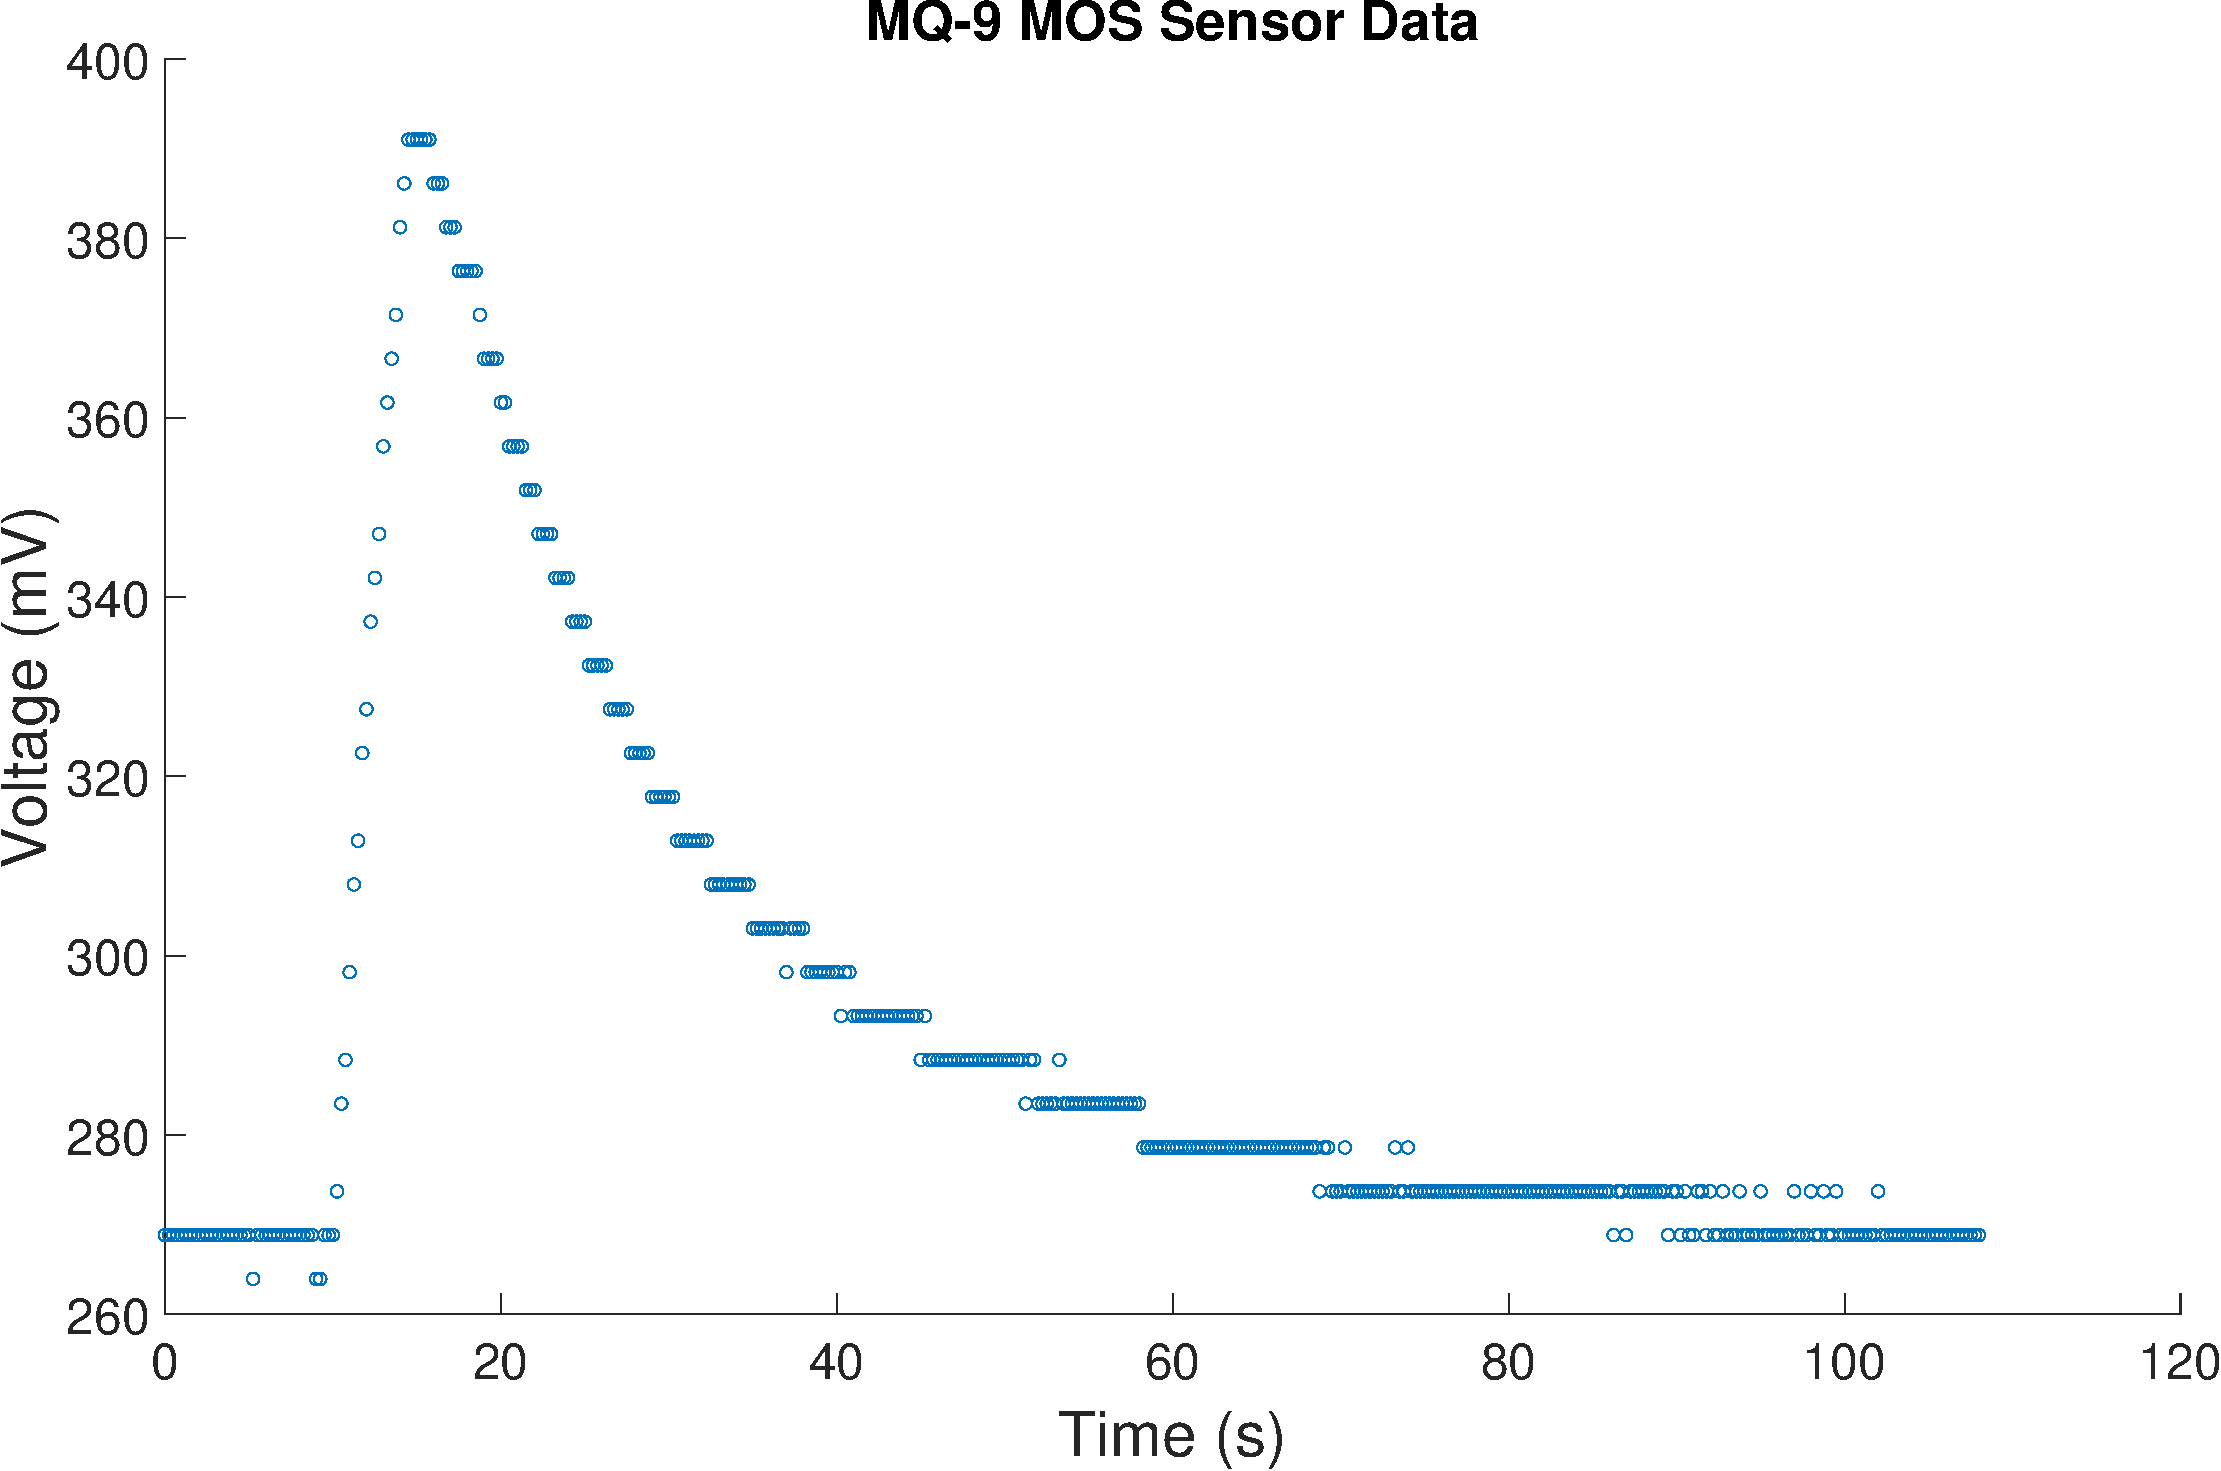
\includegraphics[width=.8\linewidth]{../figures/MQ9_MOS_Sensor_BreathEvent_Hysteresis}
    \caption{The response curve of the MQ-9 MOS sensor is shown. In the figure, the 4.5 seconds of breath are seen as a large peak upwards and the recovery time is seen as the rightward tail of the peak.}
    \label{breathExp}
\end{figure}

\section{Discussion and Conclusion}

The MOS sensor is a bit more delicate than I initially thought it would be. Given the challenges in calibration and its sensitivity to temperature and humidity, I don't know if this is a great sensor for analyzing the chemical composition of the steam. Typical applications of these kinds of sensors also focus on dynamic measurements from moving sources instead of what was done here - a static measurement in a room without much air circulation. \cite{mossensornose} showed the ability of the MOS sensors to be used in the detection of liver cirrosis, but they also mention that the possible drift and ``Time-consuming recalibration'' process make these sensors more difficult to work with. As a note, the aforementioned paper also reports sensor resistances of $\sim400\text{k}\Omega$. If the goal of using the MOS sensor is to get a readout of $x$ PPM of $y$ substance, that will require a lot of work once you receive the sensor. That goal might be unachievable given the lack of selectibility of the sensor.

When finishing my research into the MOS sensor, I found there are alternative sensors that exist that \textit{may} well be the answer to the problem I'm looking to solve. The \href{https://en.wikipedia.org/wiki/Nondispersive_infrared_sensor}{Nondispersive infrared (NDIR) sensor} provides gas sensing with broadband infrared light. Some examples of these sensors are the \href{https://www.mouser.com/ProductDetail/Amphenol-Advanced-Sensors/T6793?qs=doiCPypUmgEWnHL00v9AUQ%3D%3D}{T6793} (\href{https://www.mouser.com/catalog/specsheets/Amphenol_AAS-920-685G-Telaire-T6793-Series-021121-web.pdf}{datasheet}) which is an UART/I2C capable device that can be used for CO$_2$ detection and the \href{https://www.mouser.com/ProductDetail/ScioSense/APC1001U?qs=doiCPypUmgHCTKsIOs%2F1sA%3D%3D}{APC1001U} (\href{https://www.mouser.com/datasheet/3/3760/1/F4DCC5BD4DE584B79473B14E3148B6481EBB75469C57982156B0D6B623653729.pdf}{datasheet}) - another UART/I2C device \underline{with 3.3V communication interface} - which can be used to detect, among other things, air quality index, temperature, humidity, and ``equivalent CO$_2$ values''. These sensors may be a better alternative to MOS sensors if they prove to delicate for gas analysis.

While there are major shortcomings of the MOS sensor, its main point of strength is its sensitivity. The results seen in Figure \ref{breathExp} were quite surprising in that a ``quick and dirty'' test of my breath was able to illicit a strong signal response in the sensor. Detecting gas concentration \textit{changes} appears to be a very strong point of the sensors and might still make them useful.

\end{document}

%==================Figure==================%
\begin{figure}[h!]
    \centering
    \includegraphics[width=.8\linewidth]{p51}
    \caption{This figure shows .}
    \label{p4}
\end{figure}
%================Side-by-Side Figures================%
\begin{figure}[h!]
\centering
\begin{subfigure}{.5\textwidth}
  \centering
  \includegraphics[width=.6\linewidth]{p31}
  \caption{CAPTION}
  \label{LABEL1}
\end{subfigure}%
\begin{subfigure}{.5\textwidth}
  \centering
  \includegraphics[width=.6\linewidth]{p32}
  \caption{CAPTION}
  \label{LABEL2}
\end{subfigure}
\label{LABEL}
\caption{}
\end{figure}
%==================Boxed Equations==================%
\[
    \boxed{\vec{F}_{net} = m \vec{\ddot{r}}}
\]
%==================alphabetic enumeration==================%
\begin{enumerate}[label=(\alph*)]
    \item 
\end{enumerate}